\subsection{Alloy}
% Set Language
\lstset{
  language={alloy},
  basicstyle=\small\ttfamily, % Global Code Style
  captionpos=t, % Position of the Caption (t for top, b for bottom)
  extendedchars=true, % Allows 256 instead of 128 ASCII characters
  tabsize=2, % number of spaces indented when discovering a tab 
  columns=fixed, % make all characters equal width
  keepspaces=true, % does not ignore spaces to fit width, convert tabs to spaces
  showstringspaces=false, % lets spaces in strings appear as real spaces
  breaklines=true, % wrap lines if they don't fit
  frame=trbl, % draw a frame at the top, right, left and bottom of the listing
  frameround=tttt, % make the frame round at all four corners
  framesep=4pt, % quarter circle size of the round corners
  numbers=left, % show line numbers at the left
  numberstyle=\color{numbersRed}\tiny\ttfamily, % style of the line numbers
  commentstyle=\color{eclipseGreen}, % style of comments
  keywordstyle=\color{eclipsePurple}, % style of keywords
  stringstyle=\color{eclipseBlue}, % style of strings
}
We have used the functionalities provided by the Alloy tool in order to represent the domain assumptions of our System. 
The model, as we will see, represents a snapshot of the System at a given time.
All the interesting part of the code are commented in order to better explain their meaning.

We have also added some interesting predicates to show some possible world which is not in contrast with our assumptions.

Also, in our model we have used the \textit{Point} set in order to represents the position of interesting objects in the world. As we can easily guess, both Parking Areas and Cars are defined by a non empty set of points.

On the other hand, we have simplified our model assuming that a Person is represented by a single Point.


\subsubsection{Code}
	\lstinputlisting{../Alloy/Exported/Persons.als}
\lstinputlisting{../Alloy/Exported/Cars.als}
\lstinputlisting{../Alloy/Exported/Areas.als}
\lstinputlisting{../Alloy/Exported/GeoUtilities.als}

\subsubsection{Worlds}

\begin{figure}[!htbp]
\centering
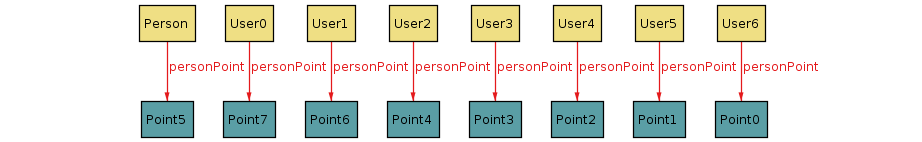
\includegraphics[width=\linewidth,keepaspectratio]{../Alloy/Exported/Images/Persons.png}
\caption{Persons}
\label{fig:Persons}
\end{figure}
As we can see from Figure \ref{fig:Persons}, we associate a single point to each person of our world.

\begin{figure}[!htbp]
\centering
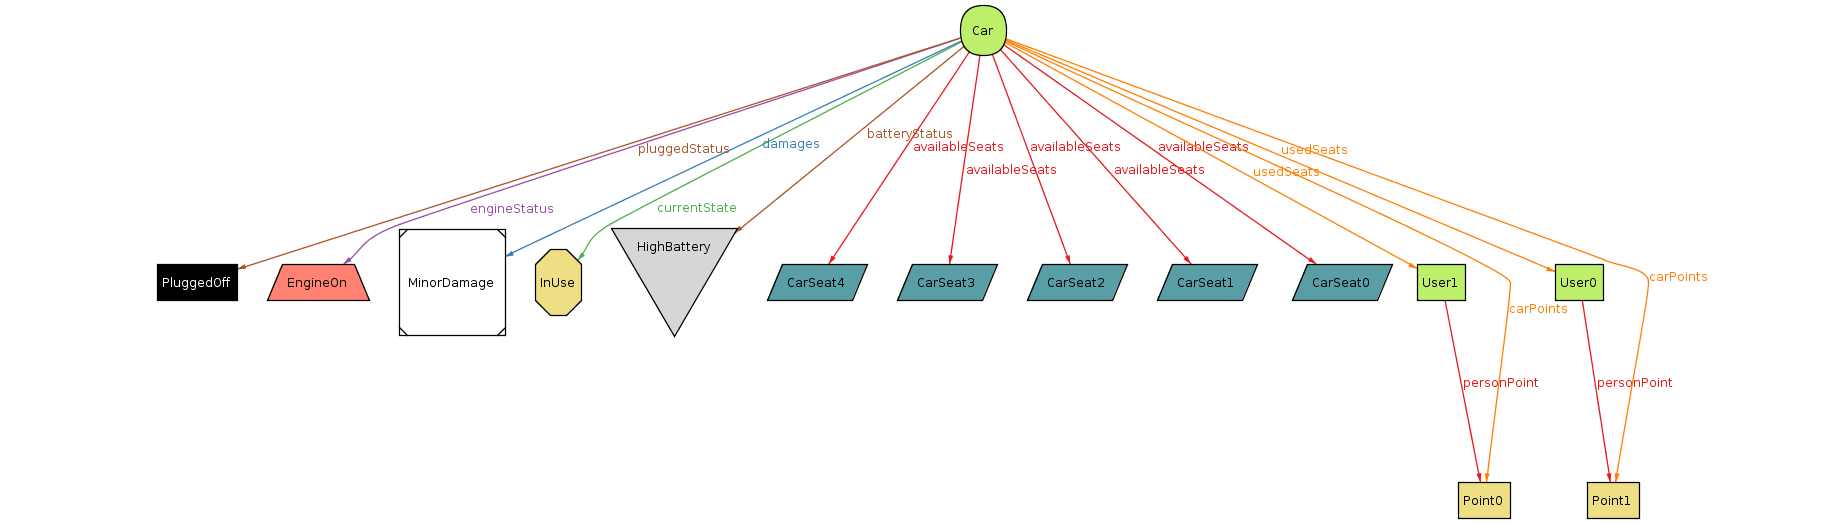
\includegraphics[width=\linewidth,keepaspectratio]{../Alloy/Exported/Images/Cars_1.png}
\caption{Example of cars}
\label{fig:Cars1}
\end{figure}
\FloatBarrier
The example in Figure \ref{fig:Cars1} represent a possible world. As we can see, the Car represented is In Use, Plugged Off and with two Users occupying two of its five seats. Also, as we can see from the Position link, the Users are both inside the Car. 

As we have previously said, this is not always the case: a Car, in our System, can be In Use, but with no person inside it. The world for this scenario is represented in Figure \ref{fig:CarsNoneInside}. Another interesting aspect shown in this image is that, although no one is inside the Car, its engine is still on.

\begin{figure}[!htbp]
\centering
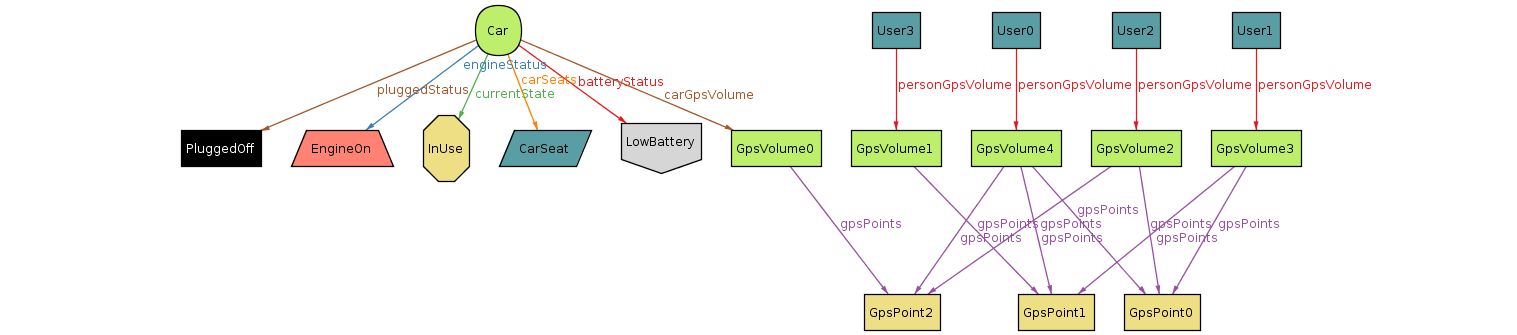
\includegraphics[width=\linewidth,keepaspectratio]{../Alloy/Exported/Images/Cars_NoPersonInsideInUseCar.png}
\caption{Used cars with no person inside}
\label{fig:CarsNoneInside}
\end{figure}
\FloatBarrier

Another meaningful aspect of our System is the possibility to have perfectly functioning cars whose status is Unavailable. This is surely due to some external Employee who have manually set the status of the Car for whatever reason. This world is shown in Figure \ref{fig:PerfectCarsUnavailable}. 

\begin{figure}[!htbp]
\centering
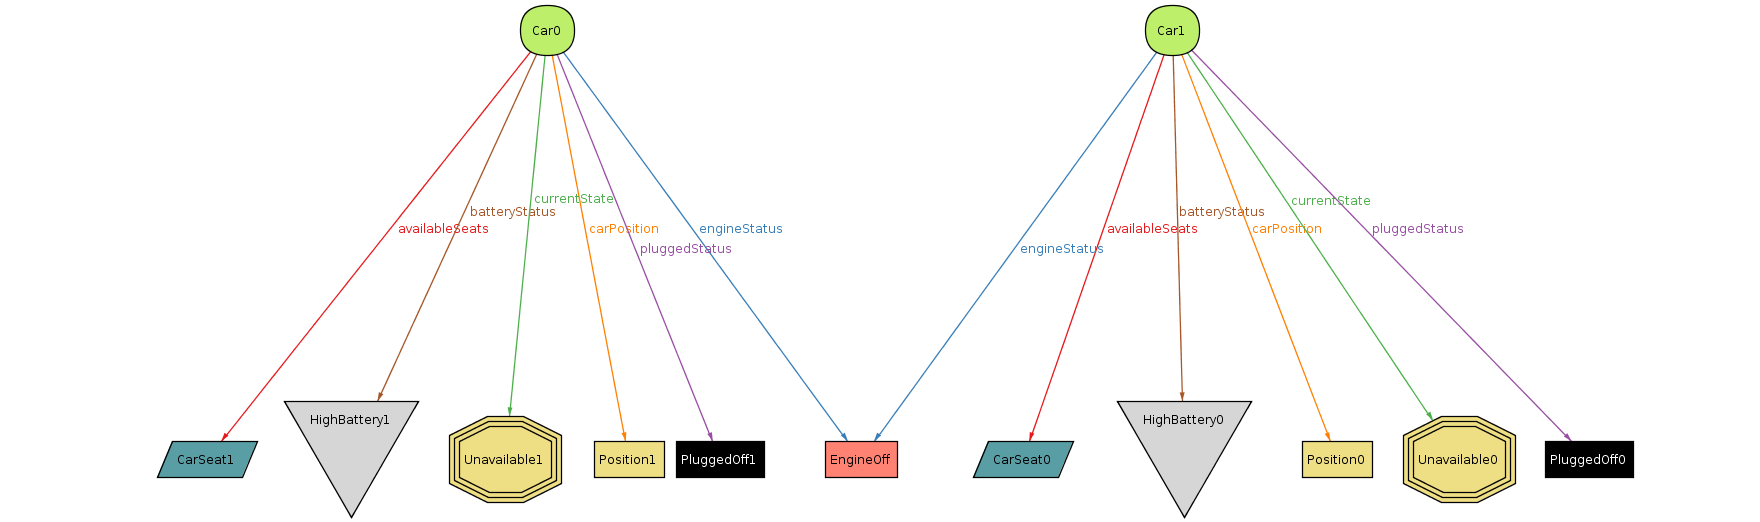
\includegraphics[width=\linewidth,keepaspectratio]{../Alloy/Exported/Images/UnavailableFunctioningCars.png}
\caption{Unavailable functioning cars}
\label{fig:PerfectCarsUnavailable}
\end{figure}
\FloatBarrier

In the successive examples, we can see how things get complicated when we add Company Areas. In Figure \ref{fig:Area1} we show a Car which is In Use and at the same time inside a Charging Area without occupying any of its charging slots. This does not come as a surprise: an User can still be inside an Area even if he/she is using the Car.

Figure \ref{fig:Area2}, instead, shows a Charging Area with a Car inside it. Differently from the previous example, in this world the Car is among the Charging Slots of the Charging Area. Its status, however, is Unavailable.

It is interesting to note the presence of a person inside the Charging Area.

\begin{figure}[!htbp]
\centering
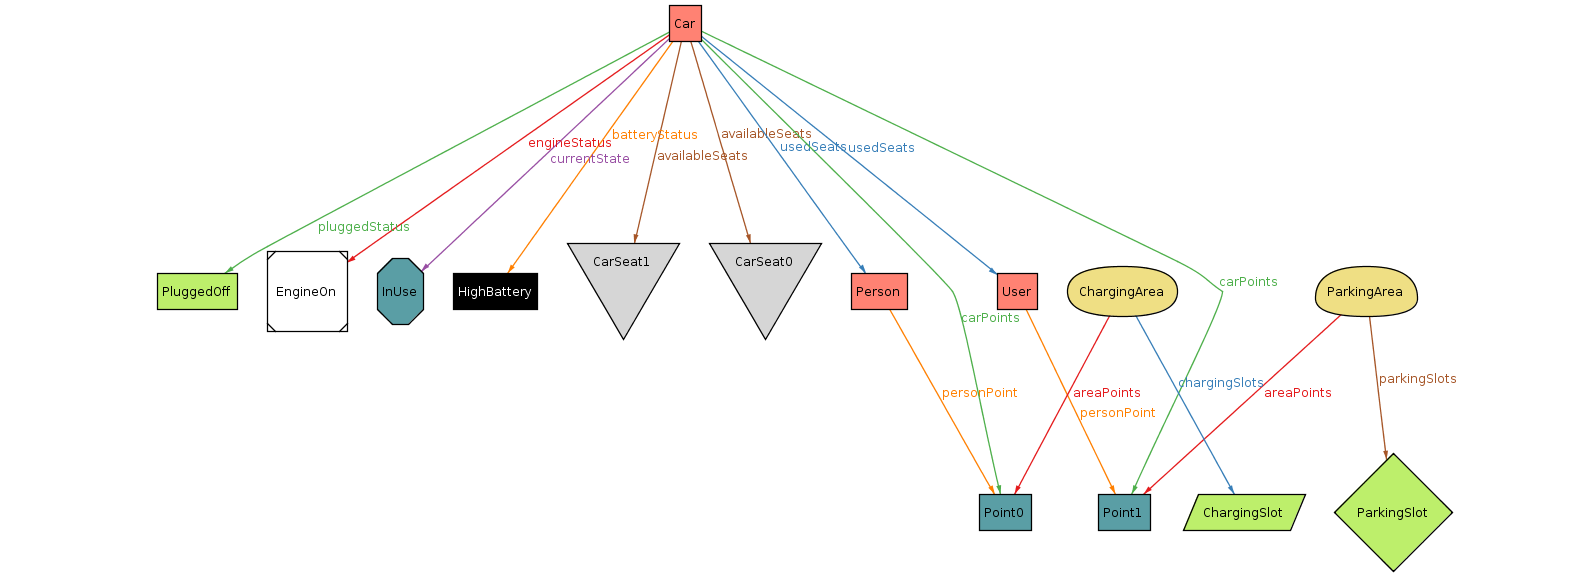
\includegraphics[width=\linewidth,keepaspectratio]{../Alloy/Exported/Images/Areas_1.png}
\caption{File Areas 1.png}
\label{fig:Area1}
\end{figure}
\FloatBarrier

\FloatBarrier
\begin{figure}[!htbp]
\centering
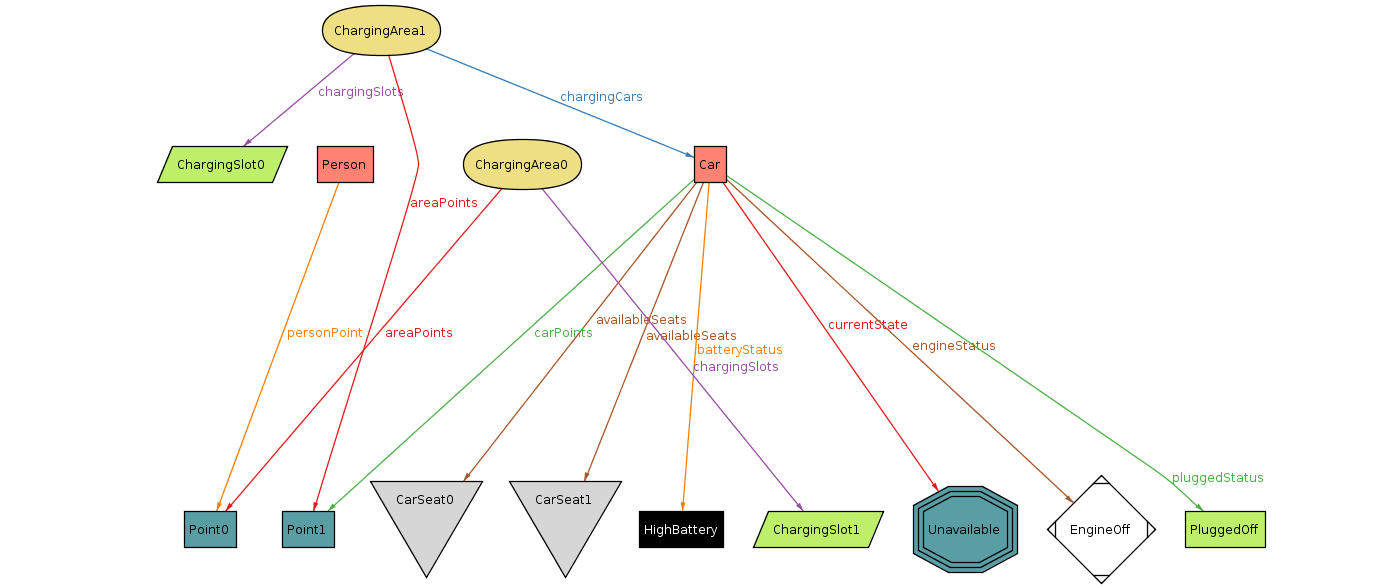
\includegraphics[width=\linewidth,keepaspectratio]{../Alloy/Exported/Images/Areas_2.png}
\caption{File Areas 2.png}
\label{fig:Area2}
\end{figure}
\FloatBarrier

\subsubsection{Executions}
In this section we simply shows that the executions of all checks in the different files have not shown the presence of counterexamples. On the other hand, the show predicates have always return valid instances. We may safely assume that our representation of the world under analysis is coherent.

\begin{figure}[!htbp]
\centering
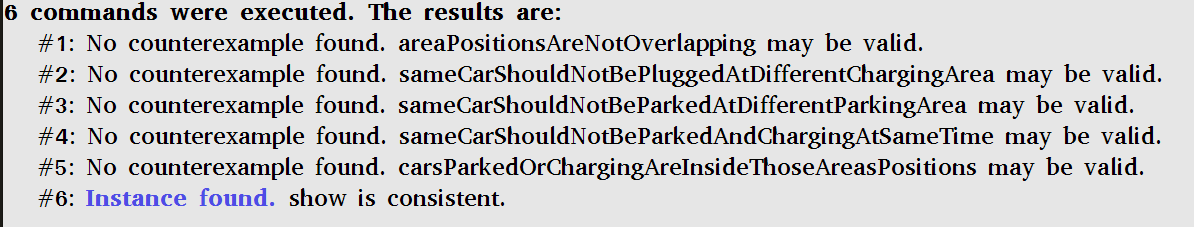
\includegraphics[width=\linewidth,keepaspectratio]{../Alloy/Exported/Images/Areas_Execute.png}
\caption{File Areas Execute.png}
\end{figure}
\FloatBarrier
\begin{figure}[!htbp]
\centering
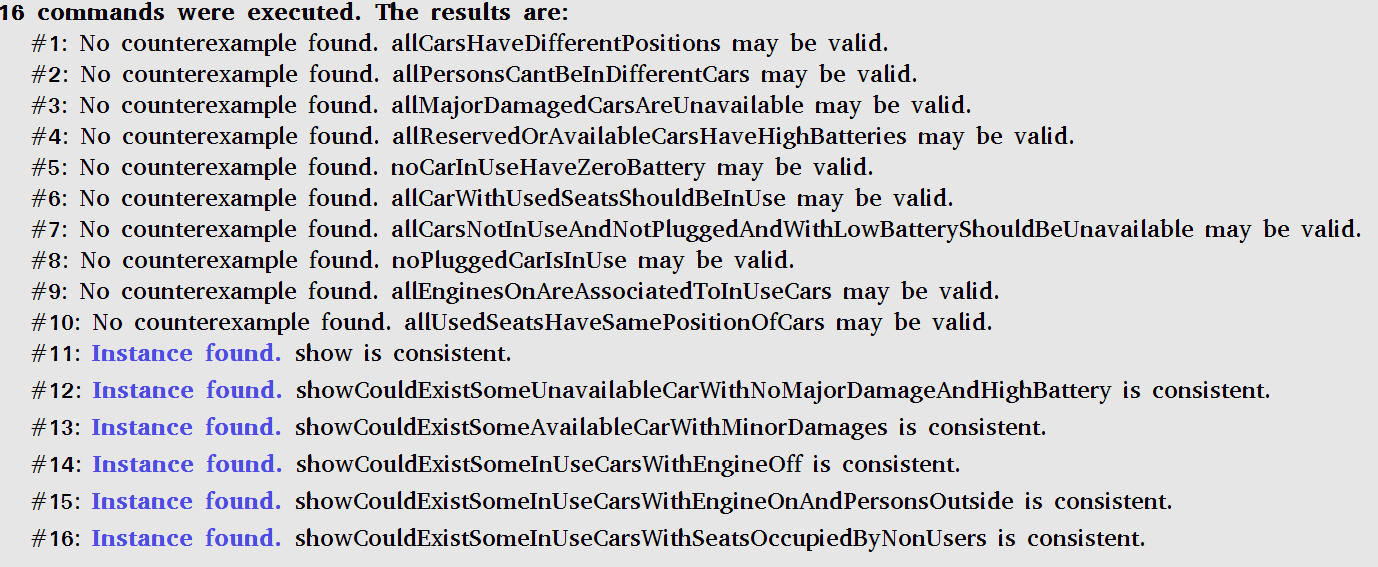
\includegraphics[width=\linewidth,keepaspectratio]{../Alloy/Exported/Images/Cars_Execute.png}
\caption{File Cars Execute.png}
\end{figure}
\FloatBarrier
